% Gemini theme
% https://github.com/anishathalye/gemini

\documentclass[final]{beamer}

% ====================
% Packages
% ====================

\usepackage[T1]{fontenc}
\usepackage{lmodern}
\usepackage[size=custom,width=120,height=72,scale=1.0]{beamerposter}
\usetheme{gemini}
\usecolortheme{gemini}
\usepackage{graphicx}
\usepackage{booktabs}
\usepackage{tikz}
\usepackage{pgfplots}
\pgfplotsset{compat=1.14}

\usepackage{fec}

% ====================
% Lengths
% ====================

% If you have N columns, choose \sepwidth and \colwidth such that
% (N+1)*\sepwidth + N*\colwidth = \paperwidth
\newlength{\sepwidth}
\newlength{\colwidth}
\setlength{\sepwidth}{0.025\paperwidth}
\setlength{\colwidth}{0.3\paperwidth}

\newcommand{\separatorcolumn}{\begin{column}{\sepwidth}\end{column}}

% ====================
% Title
% ====================

\title{Warm Starting Series of Mixed-Integer Linear Programs with Fixed Coefficent Matrices}

\author{Sean Kelley \inst{1}}

\institute[shortinst]{\inst{1} Lehigh University, Department of Industrial and Systems Engineering}

% ====================
% Footer (optional)
% ====================

\footercontent{
  \href{https://github.com/spkelle2/warm_starting_series_of_MILPs}{https://github.com/spkelle2/warm\_starting\_series\_of\_MILPs} \hfill
  ENGR 430 Final Project  \hfill
  \href{mailto:sek519@lehigh.edu}{sek519@lehigh.edu}}
% (can be left out to remove footer)

% ====================
% Logo (optional)
% ====================

% use this to include logos on the left and/or right side of the header:
\logoright{
\includegraphics[height=7cm]{lehigh_crest.jpeg}}
% \logoleft{\includegraphics[height=7cm]{logo2.pdf}}

% ====================
% Body
% ====================

\begin{document}

\begin{frame}[t]
\begin{columns}[t]
\separatorcolumn

\begin{column}{\colwidth}

  \begin{block}{Motivation}

		Many important classes of mixed-integer programs have solution methods that involve solving a series of Mixed-Integer Linear Programs (MILPs) with fixed coefficient matrices.
		\begin{itemize}
			\item Stochastic Dual Decomposition for MILP
			\item Branch and Price
			\item Multi-Objective MILP
			\item Bilevel MILP
		\end{itemize}
		Within such series, solvers can leverage what they discover solving one MILP to more quickly solve another (a.k.a. "Warm Start").
		
		Warm starting would enable greater performance and expand the space of tractable problems for those solved as a series of MILPs with fixed coefficient matrices.

  \end{block}

  \begin{block}{Example Instances}
	Consider MILPs (\ref{left}) and (\ref{right}) sharing the same coefficient matrix. Their respective formulations and possible Branch-and-Bound trees are below.
    \begin{columns}[T]
    	\begin{column}{0.45\textwidth}
    		\begin{align}
    			\begin{split}
    				\text{max} \{ &x + 4y : -\frac{x}{2} + y \leq 2, \\
    				&x + \frac{y}{2} \leq 4, (x, y) \in \Zmbb^2_+ \} 
    			\end{split}
    			\label{left}
    		\end{align}
    		\begin{figure}[h]
    			\resizebox{.45\textwidth}{!}{%
    				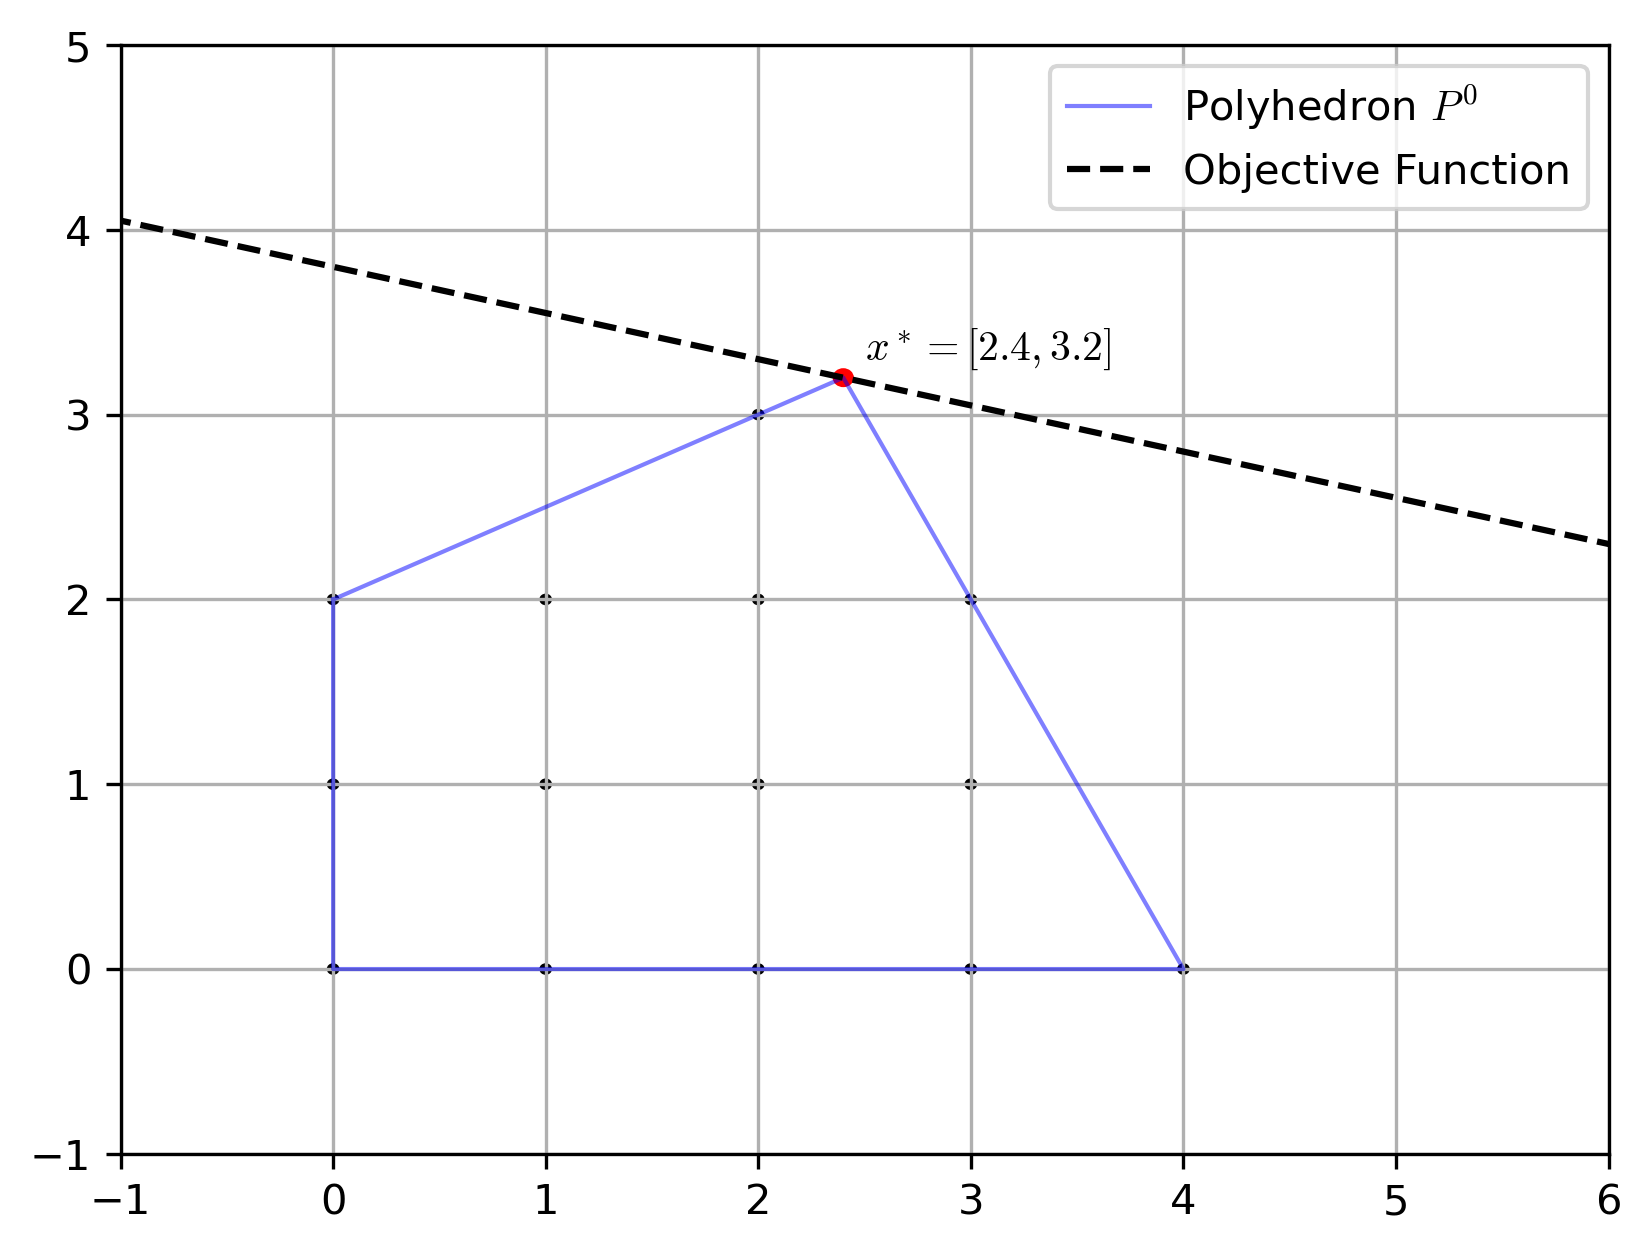
\includegraphics[]{P0.png}
    			}
    			% \caption{Node 0 LP relaxation}
    			\label{p:root}
    		\end{figure}
    		\centering
    		Branch on $ x \leq 2 $ or $ x \geq 3 $
    		\begin{figure}[]
    			\centering
    			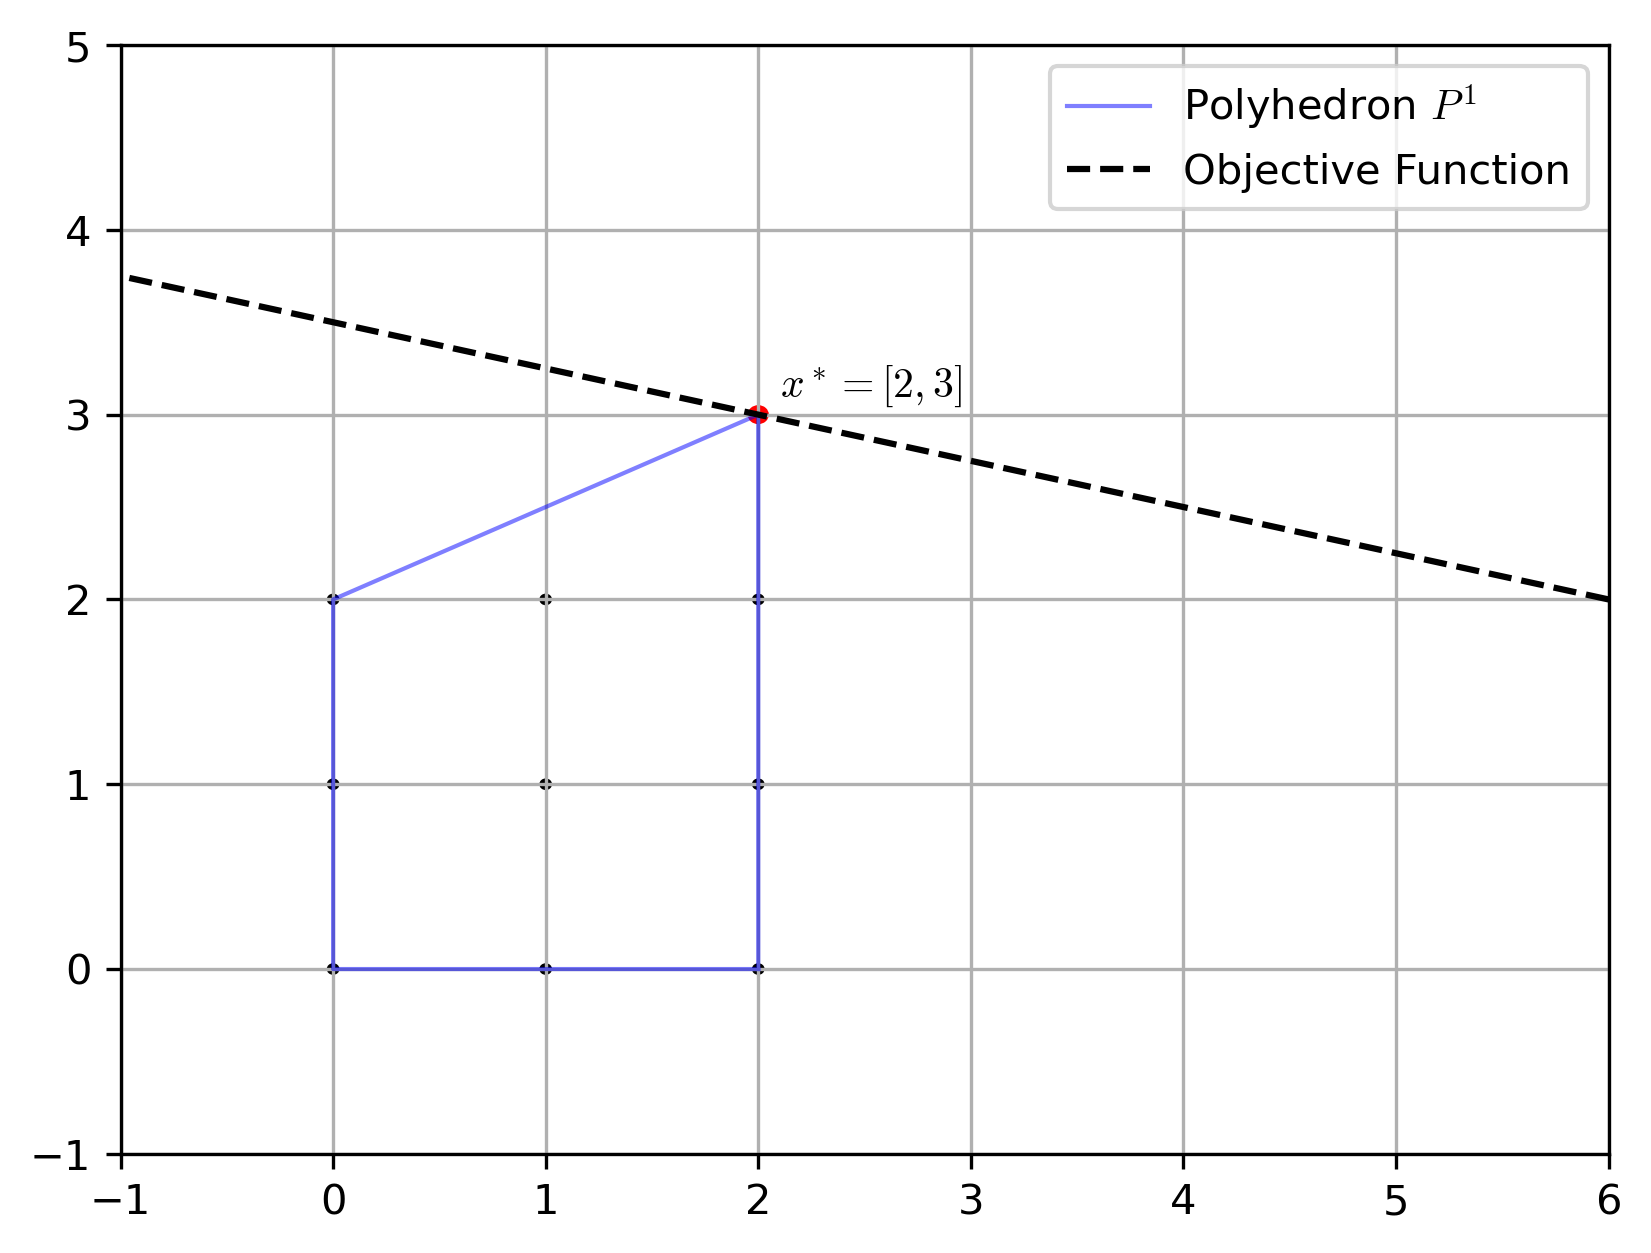
\includegraphics[width=.45\textwidth]{P1.png}
    			\hfill
    			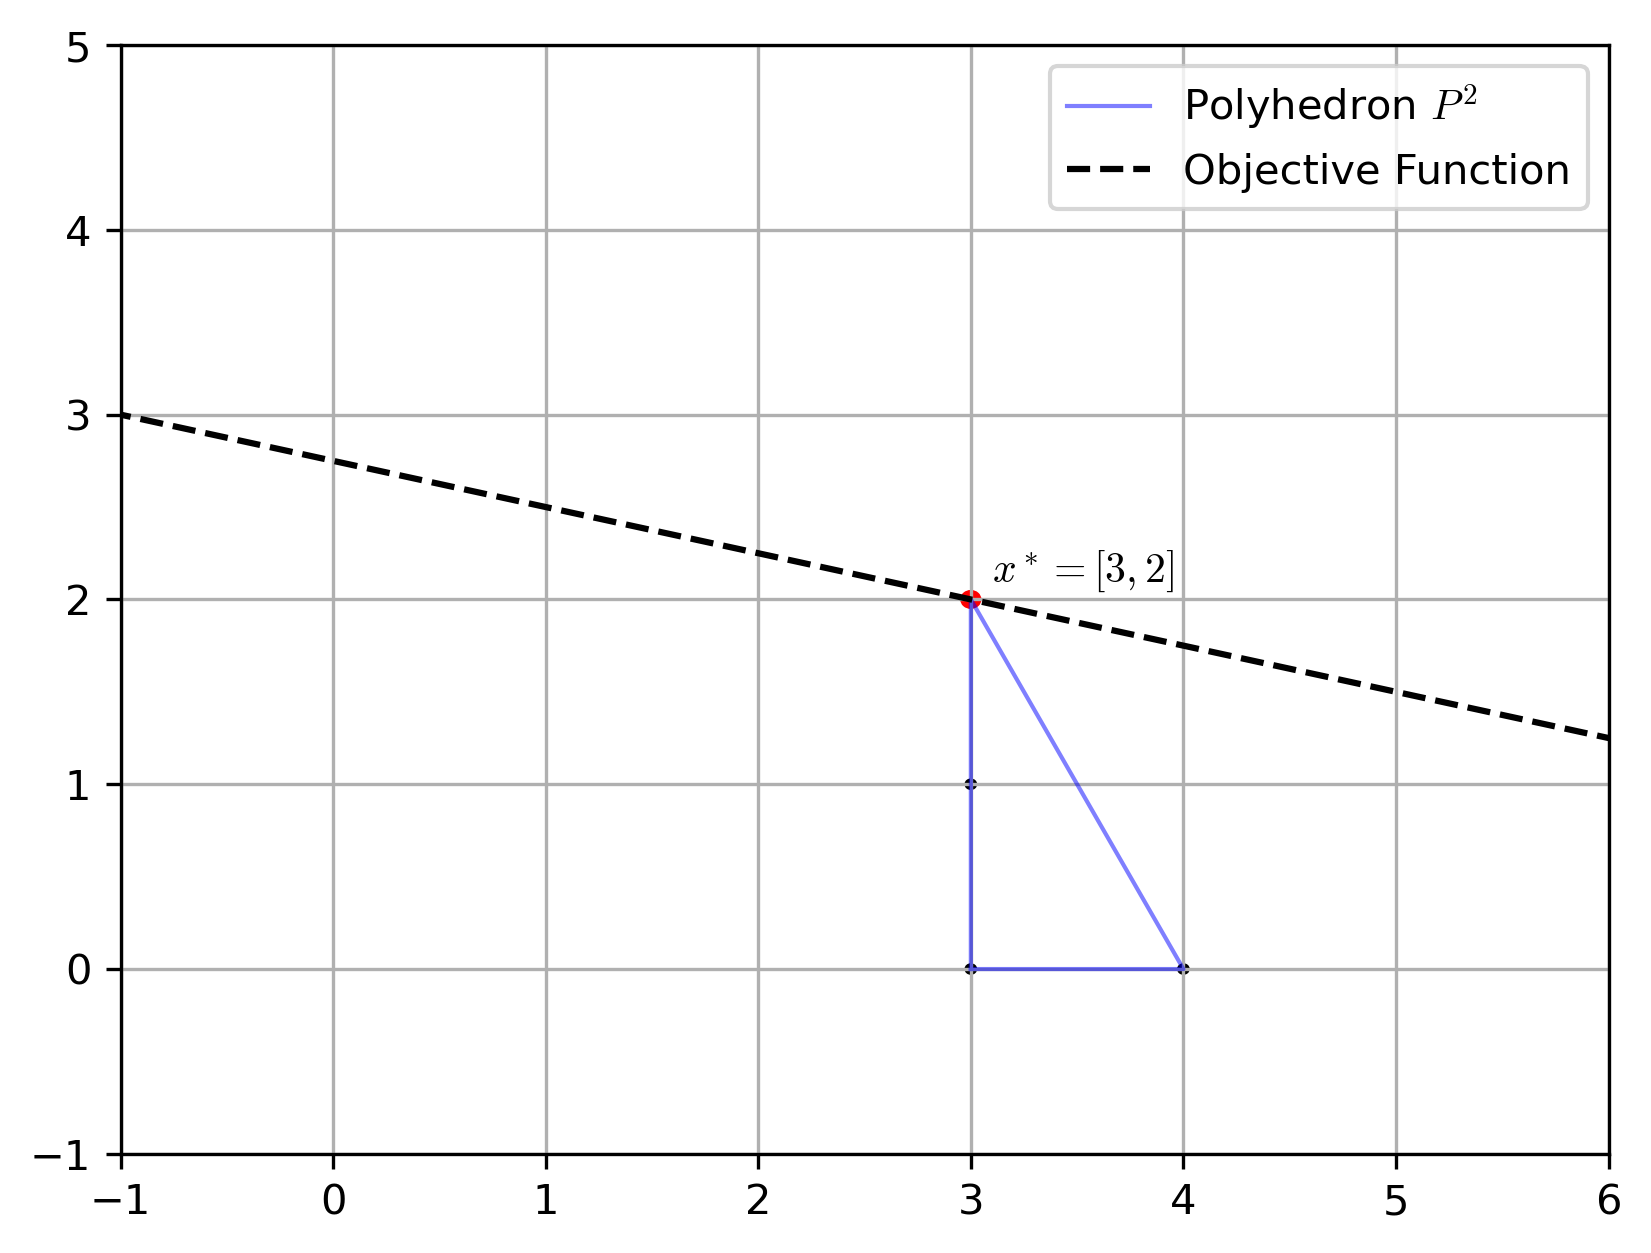
\includegraphics[width=.45\textwidth]{P2.png}
    			\caption{(\ref{left})'s Branch and Bound tree}
    			\label{p:before}
    		\end{figure}
    	\end{column}
    	\begin{column}{0.10\textwidth}
    		\vspace{7.5cm}
    		\centering
    		Update bounds $ \implies $
    	\end{column}
    	\begin{column}{0.45\textwidth}
    		\begin{align}
    			\begin{split}
    				\text{max} \{ &x + 4y : -\frac{x}{2} + y \leq 3, \\
    				&x + \frac{y}{2} \leq 5, (x, y) \in \Zmbb^2_+ \} 
    			\end{split}
    			\label{right}
    		\end{align}
    		\begin{figure}[h]
    			\resizebox{.45\textwidth}{!}{%
    				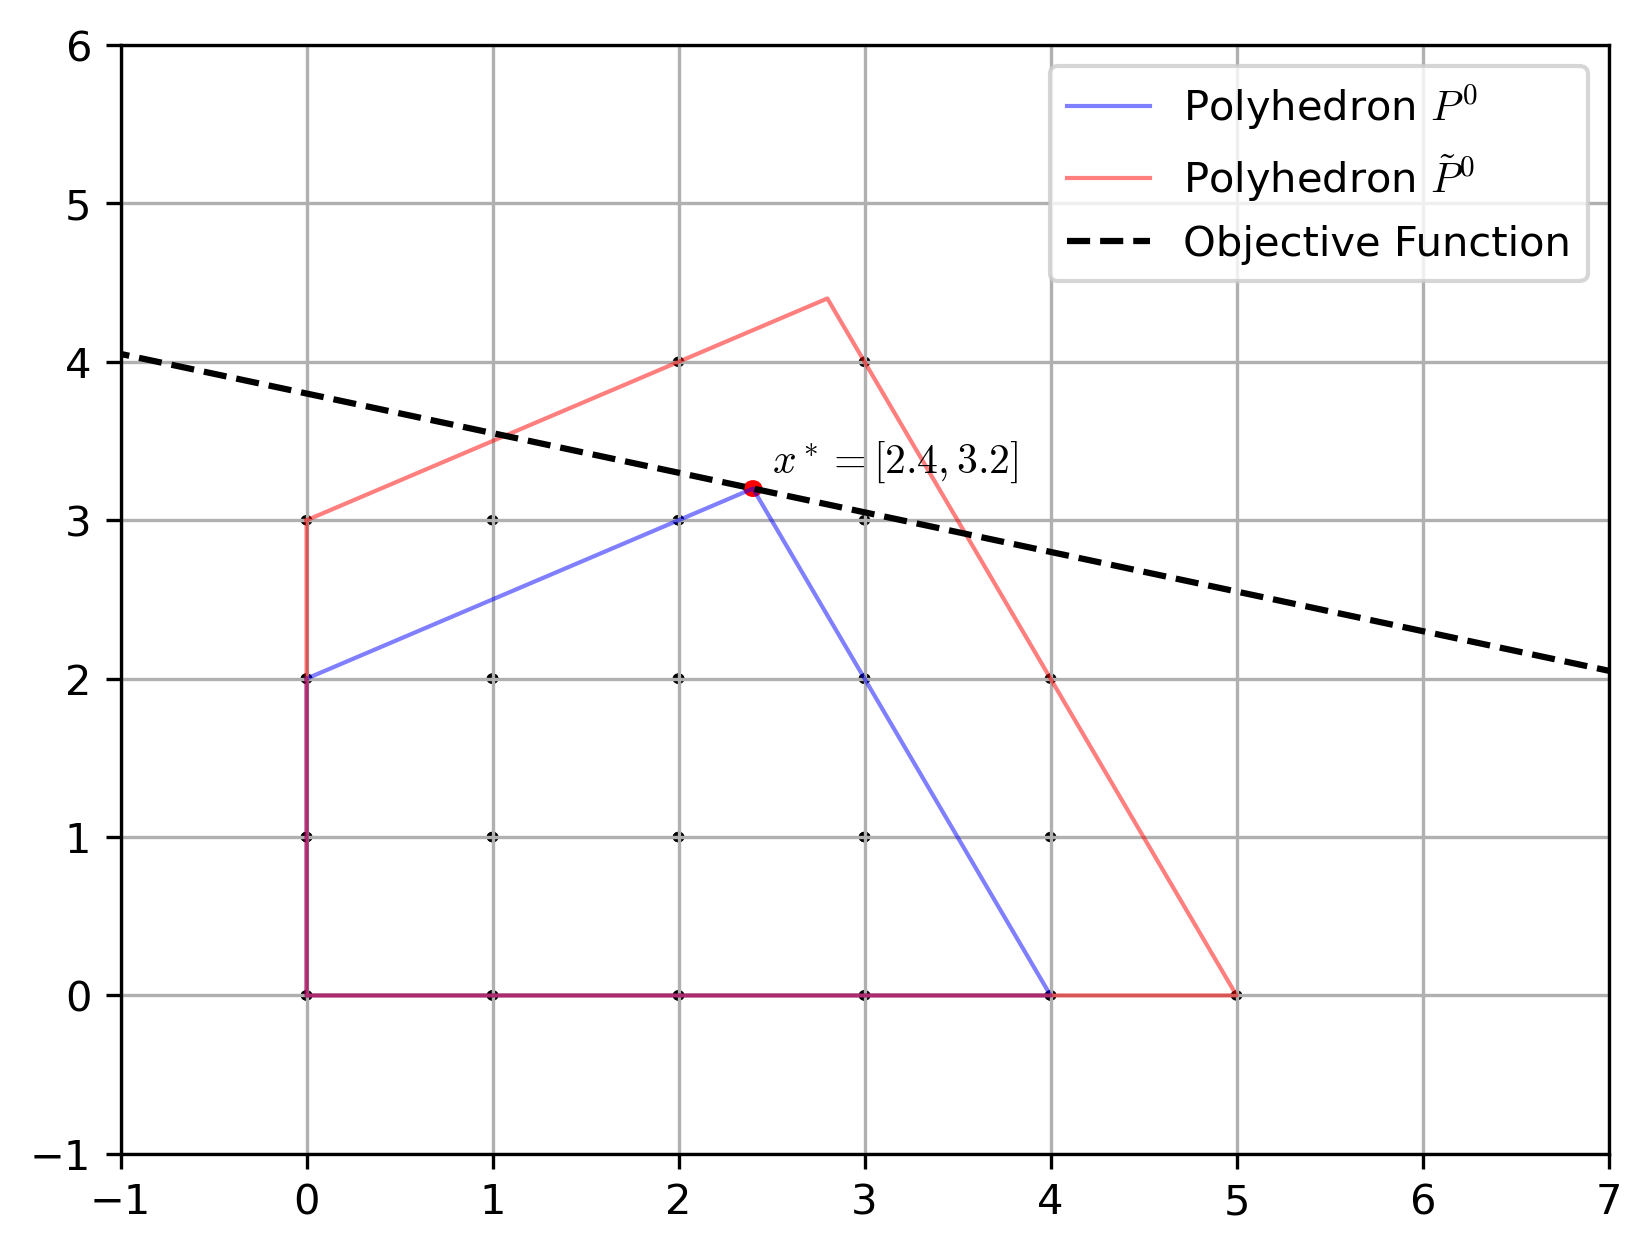
\includegraphics[]{P0_prime.png}
    			}
    			% \caption{Node 0 LP relaxation}
    			\label{p:root_prime}
    		\end{figure}
    		\centering
    		Branch on $ x \leq 2 $ or $ x \geq 3 $
    		\begin{figure}[]
    			\centering
    			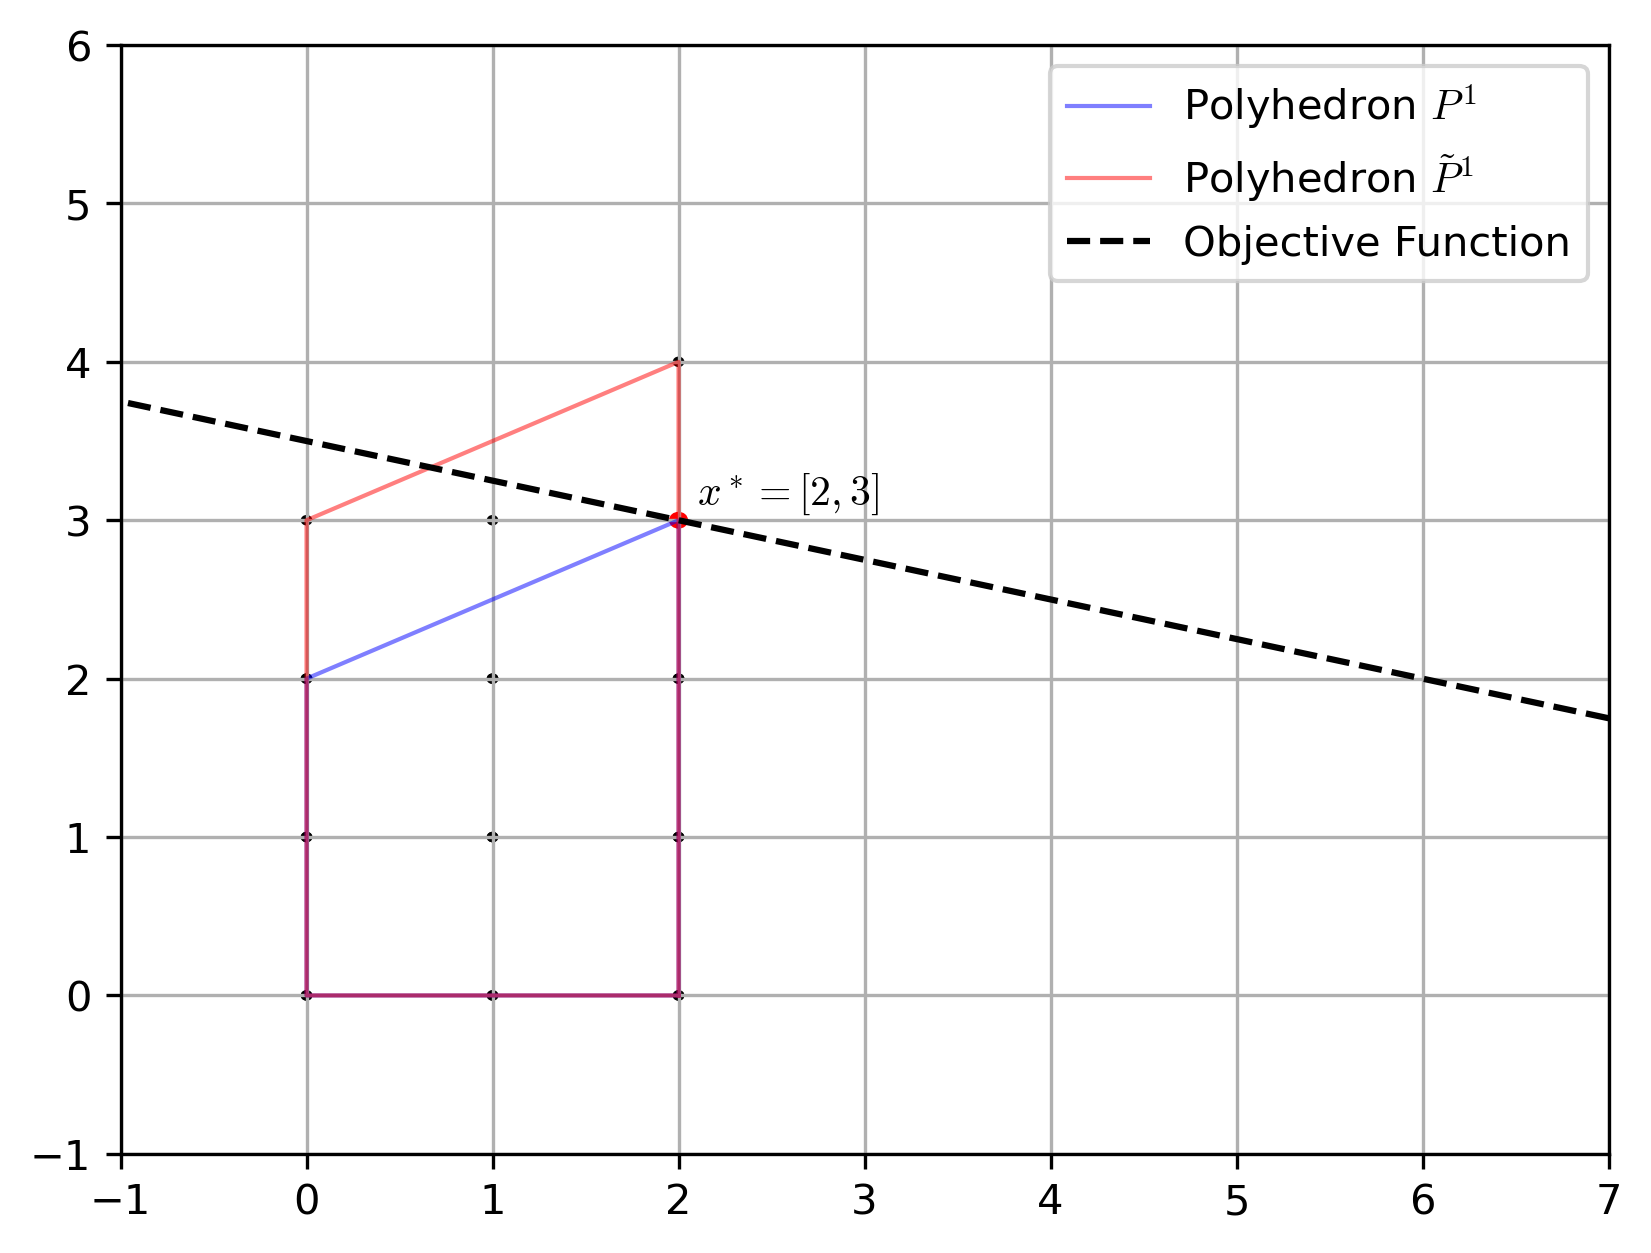
\includegraphics[width=.45\textwidth]{P1_prime.png}
    			\hfill
    			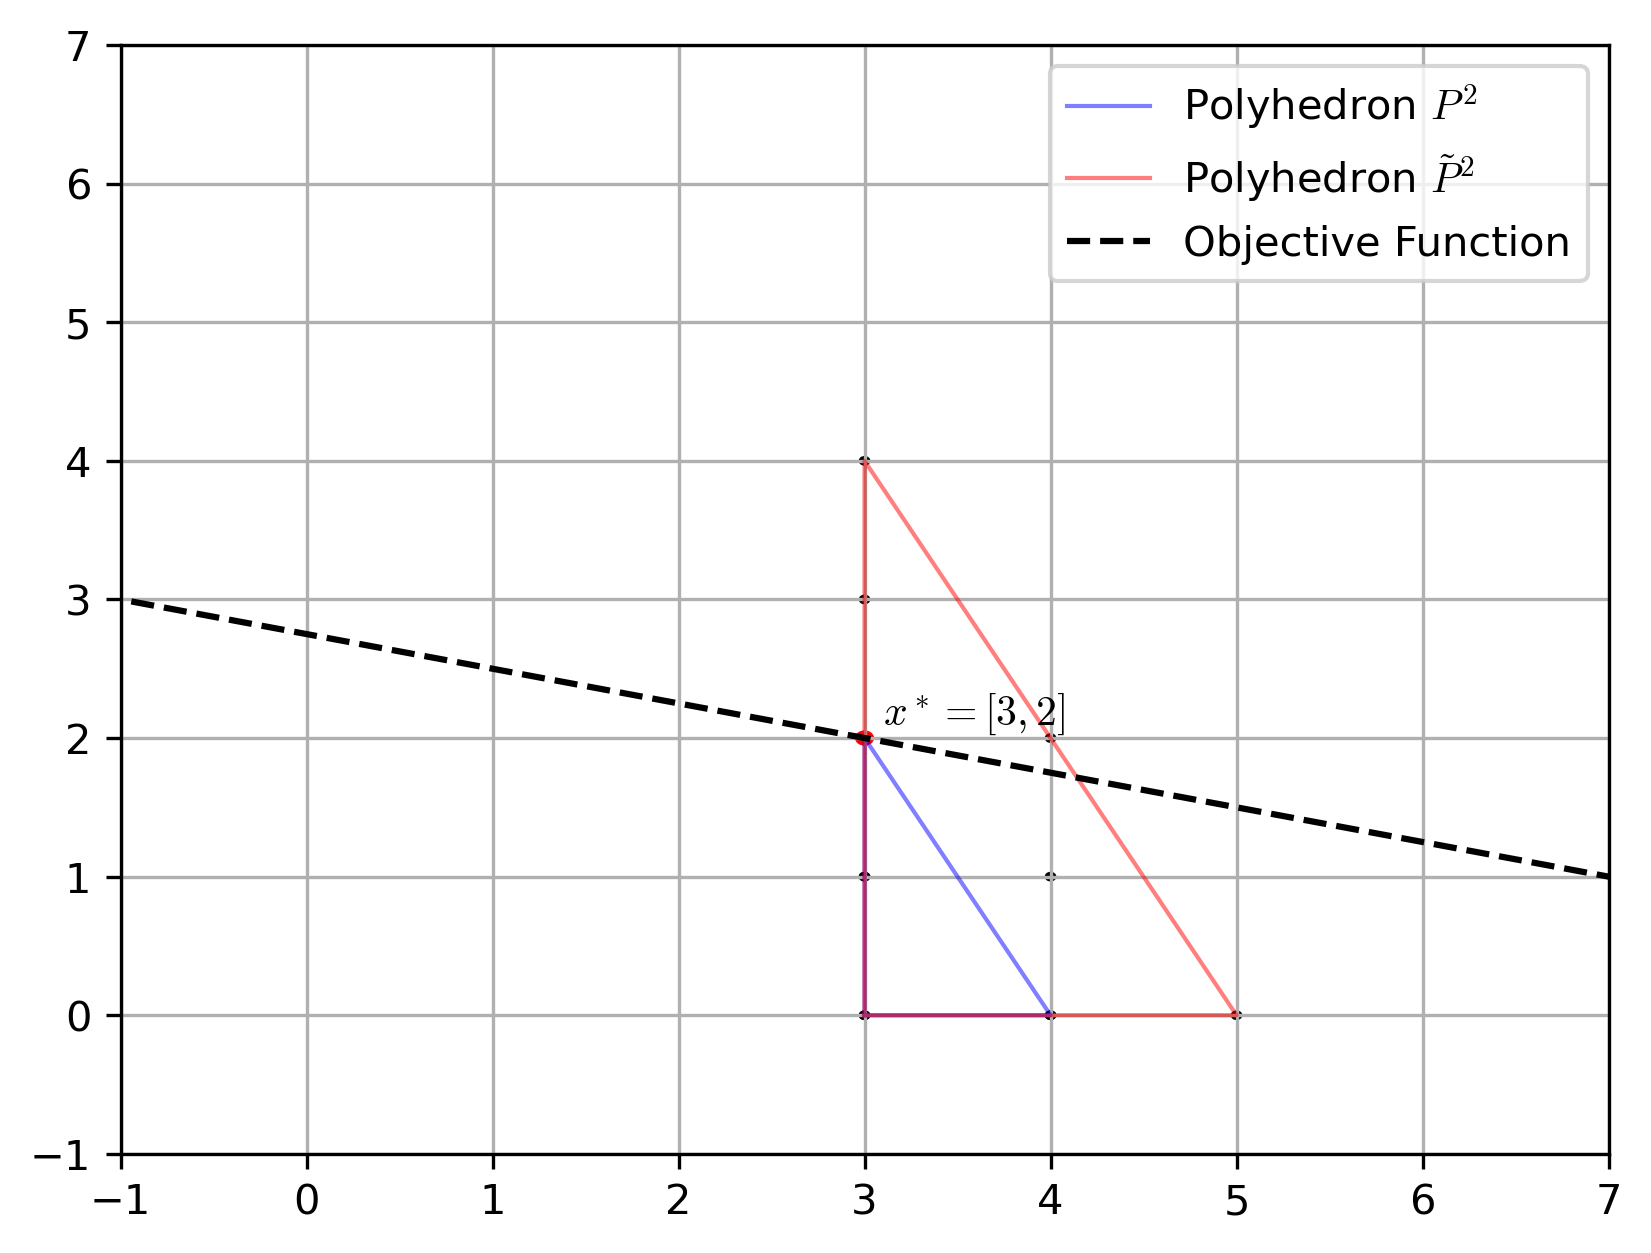
\includegraphics[width=.45\textwidth]{P2_prime.png}
    			\caption{(\ref{right})'s Branch and Bound tree}
    			\label{p:after}
    		\end{figure}
    	\end{column}
    \end{columns}
  \end{block}

  \begin{block}{Warm-Starting with Terminal Nodes of a Disjunction}

    After solving (\ref{left}), one approach to warm-start (\ref{right})'s solve is
    \begin{itemize}
    	\item Applying (\ref{left})'s disjunction to (\ref{right})
    	\item Substituting (\ref{right})'s variable and constraint bounds in each subproblem of (\ref{left}) (creating the red polyhedra from the blue).
    	\item Running Branch-and-Bound starting its queue with (\ref{right})'s terminal nodes.
    \end{itemize}
	This approach is known as \textbf{Warm-Starting with Terminal Nodes of a Disjunction}. It saves the solver from having to reprocess the root node of (\ref{right}), potentially yielding an optimal solution in less time.

  \end{block}

\end{column}

\separatorcolumn

\begin{column}{\colwidth}

  \begin{block}{Warm-Starting with Disjunctive Cuts}

    \begin{columns}[T]
    	% a cut valid for the subproblems of the second instance
    	\begin{column}{0.4\textwidth}
    		\vspace{-.25cm}
    		\begin{figure}[h]
    			\resizebox{\textwidth}{!}{%
    				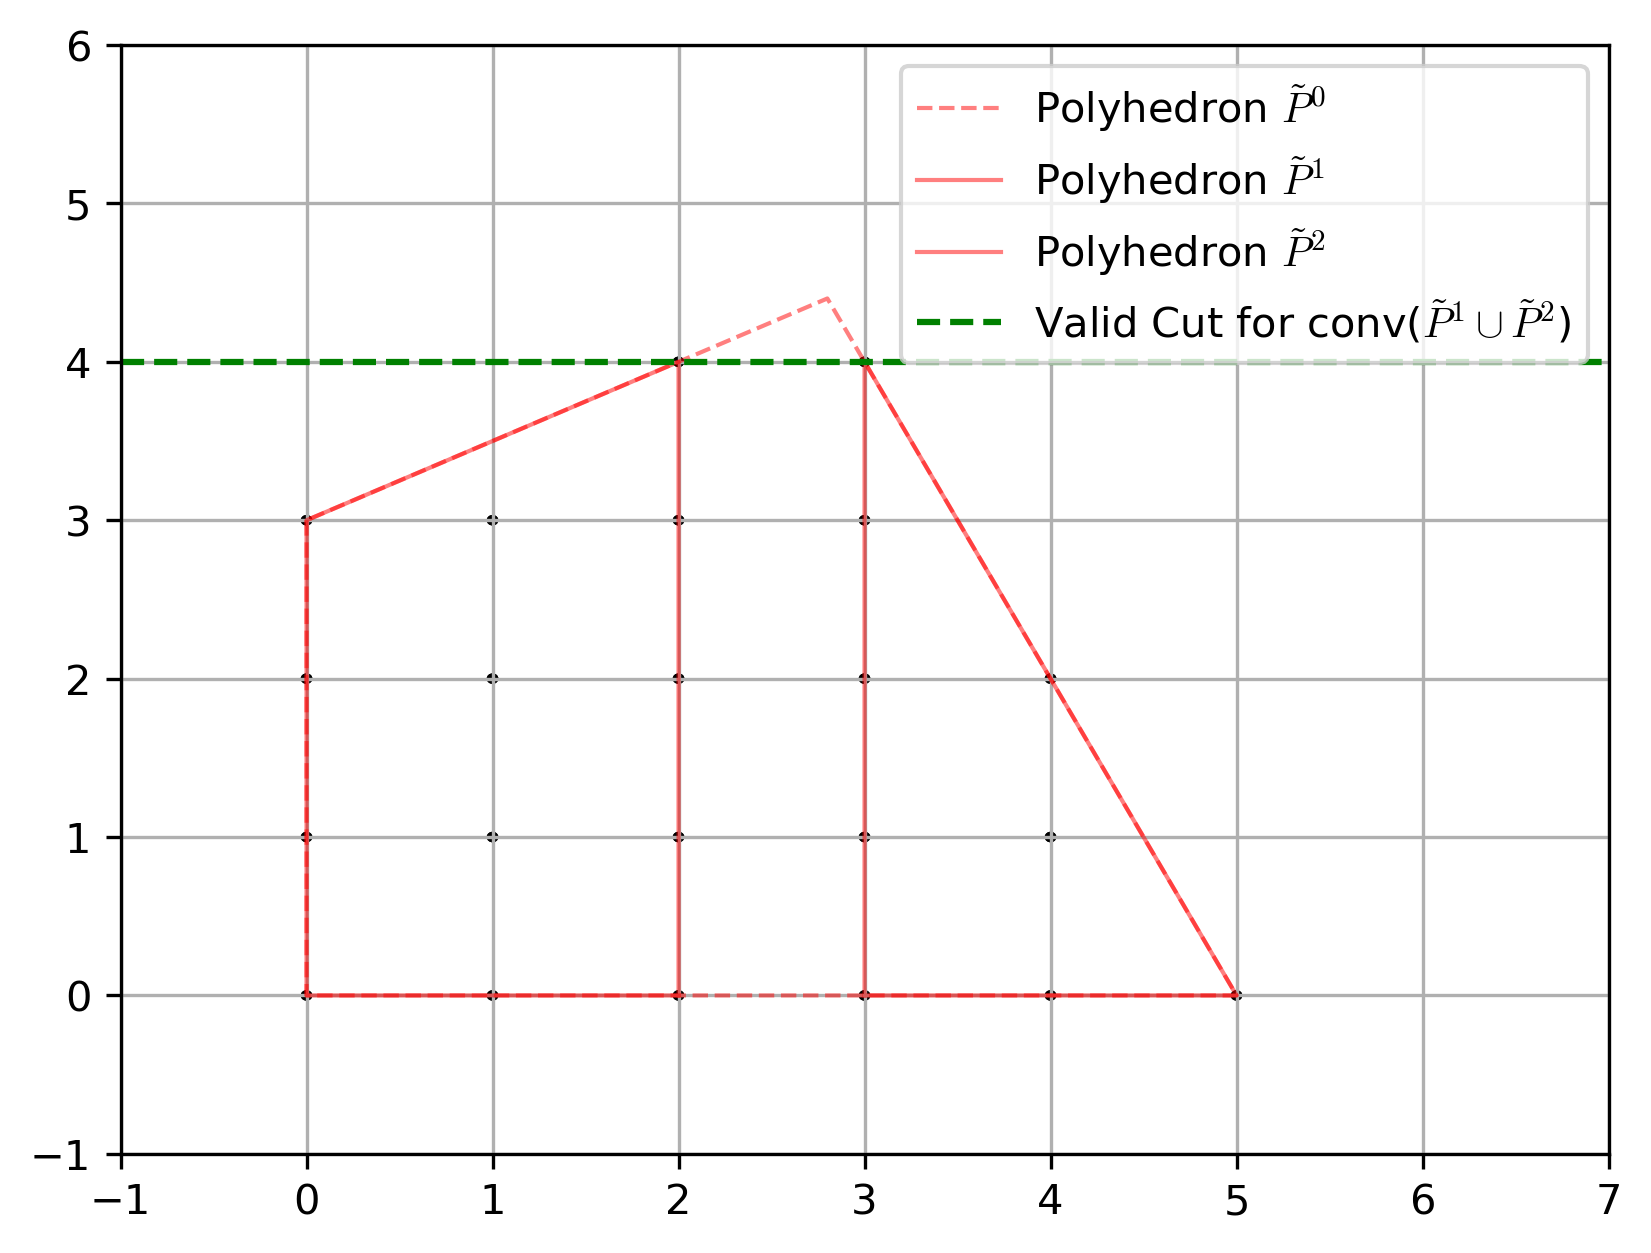
\includegraphics[]{PD_prime.png}
    			}
    			\caption{A disjunctive cut (in green) for (\ref{right})}
    			\label{p:hull}
    		\end{figure}
    	\end{column}
    	\begin{column}{0.6\textwidth}
   			Warm-starting from terminal nodes of a disjunction has drawbacks:
   			\begin{itemize}
   				\item Each terminal node must be reprocessed.
   				\item The refinement of the feasible region may occur far from the solution.
   			\end{itemize}
   			These drawbacks can be alleviated by adding \textbf{disjunctive cuts} to the root relaxation. Disjunctive cuts ensure:
   			\begin{itemize}
   				\item No terminal subproblem is violated.
   				\item Some estimate of the solution is maximally violated.
   			\end{itemize}
   			\textbf{Warm-Starting with Disjunctive Cuts} means to run Branch-and-Bound starting from the root node with an added cut generation routine to create disjunctive cuts.
    	\end{column}
    \end{columns}
  \end{block}

  \begin{block}{Disjunctive Cut Preliminaries}
  	Let MILP-$ k $ and MILP-$ l $ be solved and unsolved MILP instances, respectively, sharing a coefficient matrix. The Branch-and-Bound tree for a MILP-$ k $ has the following Linear Programming (LP) relaxation at a node $ t $:
	\begin{align}
		\begin{split}
			\text{minimize } & {c^k}^T x \\
			\text{subject to } & A^{kt}x \geq b^{kt} \\
			& u^{kt} \geq x \geq l^{kt}
		\end{split} \label{e:lp-kt} \tag{LP-$ kt $}
	\end{align}
	Above, $ A^{kt} = \begin{bmatrix} A \\ \Pi^{kt} \end{bmatrix} $, $ b^{kt} = \begin{bmatrix} b^k \\ \Pi_0^{kt} \end{bmatrix} $, ($ \Pi^{kt}, \Pi_0^{kt} $) represent constraints added from a cut generation subroutine, and $ u^{kt} $ and $ l^{kt} $ are bounds on $ x $ from branching.
	
	A Branch-and-Bound tree for MILP-$ l $ with valid LP relaxations can be generated by
	\begin{itemize}
		\item Applying the disjunction on MILP-$ k $ to MILP-$ l $.
		\item Overloading $ \Pi_0^{kt} $ to map $ b^l $ such that $ (\Pi^{kt}, \Pi_0^{kt}(b^l)) $ become valid inequalities for the solutions to MILP-$ l $ in LP-$ lt $.
	\end{itemize}
	For $ A^{lt} = \begin{bmatrix} A \\ \Pi^{kt} \end{bmatrix} $ and $ b^{lt} = \begin{bmatrix} b^l \\ \Pi_0^{kt}(b^l) \end{bmatrix} $, this yields the following formulation for a LP relaxation of MILP-$ l $ at node $ t $.
	\begin{align}
		\begin{split}
			\text{minimize } & {c^l}^T x \\
			\text{subject to } & A^{lt}x \geq b^{lt} \\
			& u^{kt} \geq x \geq l^{kt}
		\end{split} \label{e:lp-lt} \tag{LP-$ lt $}
	\end{align}
	For $ \mu^{lt} \in \Rmbb_+^{m}$, $ w^{lt} \in \Rmbb_+^{n}$, $ v^{lt} \in \Rmbb_+^{n} $, and $ I_n $ the $ n $-dimensional identity matrix, the following is a valid inequality for \ref{e:lp-lt}.
	\begin{align}
		{A^{lt}}^T \mu^{lt} + I_n w^{lt} - I_n v^{lt} \geq {b^{lt}}^T \mu^{lt} + {l^{kt}}^T w^{lt} - {u^{kt}}^T v^{kt} \label{e:lp_lt_valid_inequality} \tag{LP-$ lt $ valid inequality}
	\end{align}
	Let $ \mathcal{T}^l $ represent the terminal nodes of the Branch-and-Bound tree generated for MILP-$ l $. Let $ \pi \in \Rmbb^n $ and $ \pi_0 \in \Rmbb $ satisfy the following:
	\begin{align}
		\begin{split}
			\pi &\geq {A^{lt}}^T \mu^{lt} + I_n w^{lt} - I_n v^{lt} \\
			\pi_0 & \leq {b^{lt}}^T \mu^{lt} + {l^{kt}}^T w^{lt} - {u^{kt}}^T v^{lt}
		\end{split} \; \text{ for all } t \in \mathcal{T}^l \label{e:l_disjunctive_cut} \tag{$ l $-disjuctive cut}
	\end{align}
	By construction, \ref{e:l_disjunctive_cut} is a \ref{e:lp_lt_valid_inequality} for all $ t \in \mathcal{T}^k $.
	
  \end{block}

\end{column}

\separatorcolumn

\begin{column}{\colwidth}

  \begin{block}{Generating Disjunctive Cuts}

    For a solution estimate $ \bar{x} $ to MILP-$ l $, an $ l $-disjunctive cut $ (\pi, \pi_0) $ can be generated by solving the following LP:
    \begin{equation} \tag{CGLP-$ l(\bar{x}) $}
    	\begin{alignedat}{2} \label{e:cglp_l_xbar} 
    		\text{minimize } \; \; \qquad & \pi^T \bar{x} - \pi_0 && \\
    		\text{subject to } \qquad \pi & \geq {A^{lt}}^T \mu^{lt} + I_n w^{lt} - I_n v^{lt} && \;  t \in \mathcal{T}^l \\
    		\pi_0 & \leq {b^{lt}}^T \mu^{lt} + {l^{kt}}^T w^{lt} - {u^{kt}}^T v^{lt} && \; t \in \mathcal{T}^l \\
    		1 & = \sum_{t \in \mathcal{T}^l} \big( \sum_{j=1}^{m^t} \mu_j^{lt} + \sum_{i=1}^{n} w_i^{lt} + \sum_{i=1}^{n} v_i^{lt} \big) && \\
    		& \mu^{lt} \in \Rmbb_+^{m^t}, \; w^{lt} \in \Rmbb_+^n \; v^{lt} \in \Rmbb_+^n && t \in \mathcal{T}^l
    	\end{alignedat}
    \end{equation} 
	
  \end{block}

  \begin{block}{Numerical Experiments}
  	500 pairs (MILP-$ k $, MILP-$ l $) of MILP instances were selected for this study, where either $ b^k = b^l $ or $ c^k = c^l $. Each MILP-$ k $ was solved until 4 and 16 nodes were processed. MILP-$ l $ was solved three ways: cold started, warm-started with a disjunctive cut generator from the 4 node MILP-$ k $, warm-started with a disjunctive cut generator from the 16 node MILP-$ k $.
  	
  	The below graphs illustrate the dual gap improvement at the root node of MILP-$ l $ due to adding disjunctive cuts.
  	\vspace{-1.5cm}
	\begin{figure}[h]
		\resizebox{\textwidth}{!}{%
			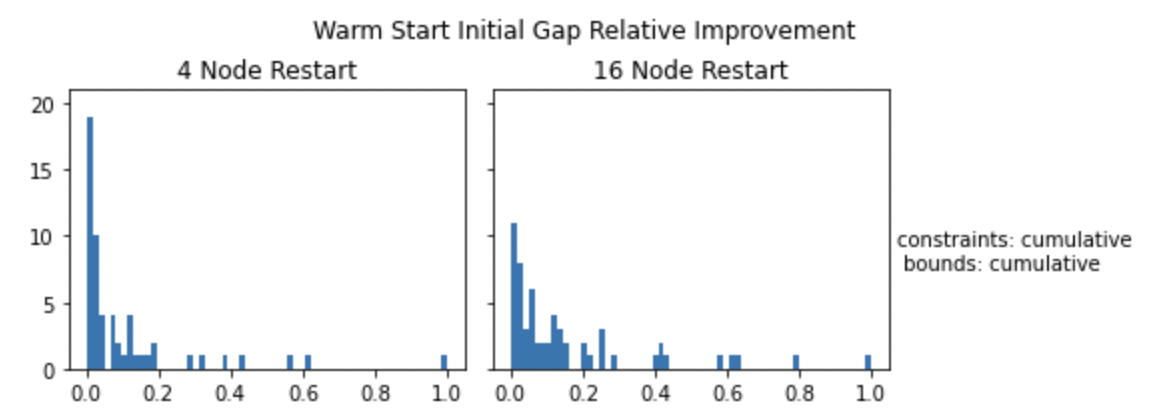
\includegraphics[]{experiment.png}
		}
		\caption{Relative dual gap improvement of root node after running disjunctive cut generator when $ b^k = b^l $}
		\label{p:experiment_fixed_b}
	\end{figure}
	\vspace{-1.5cm}
	\begin{figure}[h]
		\resizebox{\textwidth}{!}{%
			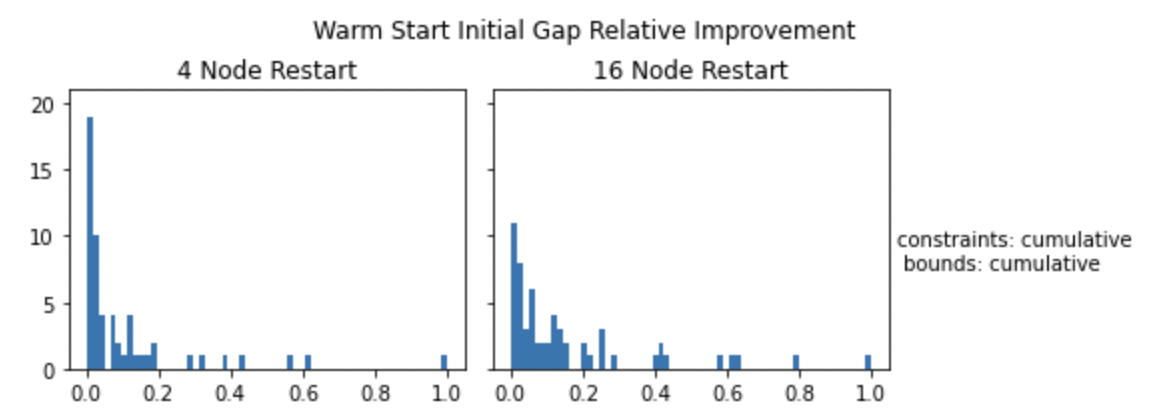
\includegraphics[]{experiment.png}
		}
		\caption{Relative dual gap improvement of root node after running disjunctive cut generator when $ c^k = c^l $}
		\label{p:experiment_fixed_c}
	\end{figure}
  \end{block}

\end{column}

\separatorcolumn
\end{columns}
\end{frame}

\end{document}
